\documentclass[10pt,a4paper]{article}
\usepackage[utf8]{inputenc}
\usepackage[english]{babel}
\usepackage{amsmath}
\usepackage{amsfonts}
\usepackage{amssymb}
\usepackage{graphicx}
\title{COS 301 Software Documentation}
\author{Dieter Doman 11002566 \\
		Melany Barnes 12030466 \\
		Rudiger Roach 11004322 \\
		Johan Esterhuyse 10043285}
\date{}
\begin{document}
\maketitle
\begin{center}
Version 1.0 \\
GitHub link: https://github.com/RudigerRoach/301\textunderscore main\textunderscore emma.git \\
\vspace*{5\baselineskip}
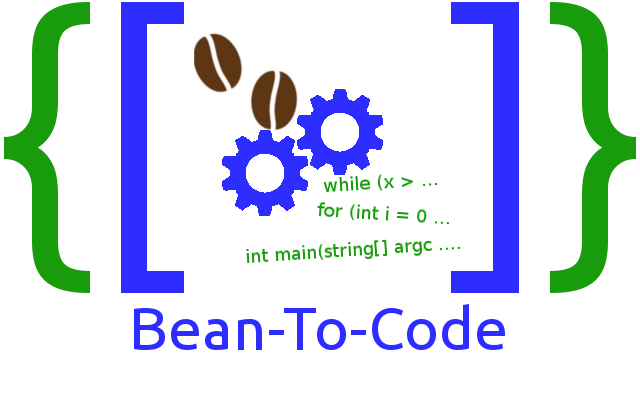
\includegraphics[scale=0.35]{Pictures/Logo.png}
\end{center}
\pagebreak
\tableofcontents
\pagebreak
\section{Vision and Scope}

\subsection{Vision}
Our client creates software for camera club event management. A big part of an event comprises of an image judging process. Currently the process is completed by us Infra-red remotes and receivers but this configuration is limiting in terms of usability and the amount of judges that can judge concurrently.\\\\
The proposed solution will replace the hardware remote with a software application to run on a mobile device. The mobile application should alleviate all of the issues caused by the current setup and should be developed with a server component that plugs into the existing EMMA system.  

\subsection{Scope}
Create a software solution that:
\begin{itemize}
\item Runs on IOS and Android mobile devices.
\item Allows as many as 20+ judges on the night.
\item Allows judges to register against the event (in order to score) by capturing an email address.
\item Remembers the scoring device for future meetings such that registration is not required again.
\item Caters for realtime scoring.
\item Can display a thumbnail image of that currently being judged.
\item Caters for simple score entry bound within a variable range.
\item Reports meaningful error messages, in a clear way.
\item Allows for quick correction and re-capture.
\item Can notify a judge of outstanding scores.
\end{itemize}

\section{Architecture requirements}
\subsection{Architecture requirements}
\subsubsection{Architectural scope}
\subsubsection{Quality requirements}
\begin{itemize}
\item Security
\paragraph{}
The systems functionality should be only available to users who can be authenticated through the EMMA system. If it is new user should be able to create new account.
\item Usability
\paragraph{}
99 percent of users should be able to easily learn how to use system without prior training.
\item Testability
\paragraph{}
All services offered by the system must be testable through unit tests which test when all pre-conditions are met that the service is provided and that all post-conditions hold true when service has been provided.
\item Performance requirements
\item Scalability
\paragraph{}
The deployed system must be able to operate effectively under the load of 30 concurrent users on single event.
\item Installability
\paragraph{}
It should be easy to install the server side component and the effort to get it running each club night should be minimal.
\end{itemize}
\subsubsection{Integration and access channel requirements}
\begin{itemize}
\item Integration requirement
\paragraph{}
The production version of this application will need to integrate with EMMA(Entry and Member Management Application). EMMA is Java based application.
\item Access channels
\paragraph{}
The mobile application will have to go through a web-service which will be and interface for the server side. 
\end{itemize}
\subsubsection{Architectural constraints}
\begin{itemize}
\item The mobile application should run on Android and iOS operating systems.
\item The PC's that will be running the server side of the application and EMMA component will generally not be the latest technology(limited memory and processing power).
\item There will be limited to no internet connection.
\item The communication between the mobile device and server PC will be done over wifi network.
\item The server side component of this project should be able to run on Windows and OS X operating systems.
\end{itemize}
\subsection{Use of reference architectures and frameworks}
\subsection{Technologies}
\begin{itemize}
\item Java
\item
\end{itemize}
\section{Functional requirements and application design}
\subsection{Introduction}
\subsection{Required Functionality}
\subsubsection{Functional requirements for registration and login}
A first time user will be required to register by filling in his/her email address and password, as well as confirm password.
To login for the first time a user will have to enter his/her email address and password. The credentials provided will be tested against the database to determine if it is valid.  If login fails the user will be directed to the register screen. If login is successful the device's unique identifier will be sent to the server to remember the device on the system. The user will then be able to use the rest of the system.

\subsection{Use case prioritization}
\subsection{Use case/Services contracts}
\subsection{Process specifications}
Activity sequence diagrams
\subsection{Domain objects}
\section{Glossary}
\end{document}